\chapter{Data Augmentation}
\label{chap:dataAug}
In this Chapter, data augmentation is introduced to control the overfitting problem. For sound type classification, there are mainly two policies for data augmentation. The effects of different data augmentation policies will also be discussed in this chapter.
\section{Overview and Motivation}
The experiment results in previous chapter show that the training of SigmoidCrossEntropy model meets the overfitting problem. Overfitting usually comes from over trained parameters. If we consider this problem in another way, that is if we have adequate training data to abstract the high level data structure, it may control the overfitting problem to a certain extent. 

Data augmentation was adopted by Krizhevsky et al. to combat the overfitting problem for ImageNet Classification.\cite{krizhevsky2012imagenet} "The easiest and most common method to reduce overfitting on image data is to artificially enlarge the dataset using label-preserving transformations."

What data augmentation does in my experiments is to randomly shift the rate maps and AMS feature over time and frequency domain. Intuitively data augmentation increase the irrelevant variability of training data, which helps the model to find a high level abstraction of the data.  Shifting over time domain only and shifting over both time and frequency domain can be seen as two shifting policies. 

However, such operation is not implemented in Caffe. In the meanwhile, Caffe provides a special type of layer, Python layer, which enables Caffe users to implement self-defined layers in python. I implemented a Python layer for the augmentation operation. The missed data values due to shifting operation are replaced by normal distributed vectors with mean and covariance matrix calculated from the original input features. Instead of padding with constant values, padding with normal distributed vectors add noise in the data rather than changing the data pattern. Such noise adds the classification irrelevant variability in the training data and hence may control the overfitting problem. The shifting step size is randomly generated in each iteration. I also set a range for the shifting steps, this range can be defined by users through the layer parameters. I experimented on a series of this range parameters. 

In the following sections, the parameter settings will be described in form $T(minT,maxT),F(minF,maxF)$. $T$ means shifting over time domain. The shifting step in each forward propagation iteration is a integer, which is uniformly distributed in range $(minT,maxT)$. One shifting step means shifting by one time frame. Positive step means shifting left, while negative step means shifting right. $F$ means shifting over frequency domain. The same as shifting over time domain, the shifting step in each forward propagation iteration over frequency domain is also a integer, which is uniformly distributed in range $(minF,maxF)$. One shifting step over frequency domain means shifting by one frequency channel. Positive step means shifting to higher frequency channels, while negative step means shifting to lower frequency channels. 


\section{Methods}
To compare the performance statistically, I carried out dependent t-tests using the 11-dimensional statistics(performance metrics) between two experiments. T-tests are widely used to determine if two sets of data are significantly different from each other. Large p-value, e.g. greater than 0.05 or 0.1,  rejects the null hypothesis of identical average scores. Small p-value smaller than the threshold, e.g. $0.01$, $0.05$,$0.1$, rejects the null hypothesis of equal averages. In this way, the comparison of performance between two experiments can be seen from this statistic, p-value.
\section{Results and Discussion}
In this section I will mainly compare the experiment results in three steps. Firstly I will compare the new model with data augmentation with the old model in previous chapter. Secondly I will compare 2 shifting policies, shifting over time domain and shifting over both time and frequency domain. At last I will compare different settings of the shifting range parameters used in the Python layer to roughly get a best setting of parameters.
\subsection{Data Augmentation effects}
\label{subsec:dataaug}
In the experiment with data augmentation, I set the shifting range to $T(-30,30)$. The other experiment result to compared with is the SigmoidCrossEntropy model from Chapter \ref{chap:architecture}. 

The experiment results are shown in Fig.\ref{fig:balcompare1}. Two vertical lines represent for the mean value lines for these two experiments. The model with data augmentation outperforms the SigmoidCrossEntropy model for most sound type classes. I also carried out a dependent t-test with the balanced accuracy statistics from these two experiments, the p-value I got is $0.049577<0.05$ which means the performance statistics of two models are indeed significantly different from each other. Data augmentation improved the model performance.
\begin{figure}[h!]
	\caption{Balanced accuracy of two models, shift over T(-30,30)}
	\label{fig:balcompare1}
	\centering
	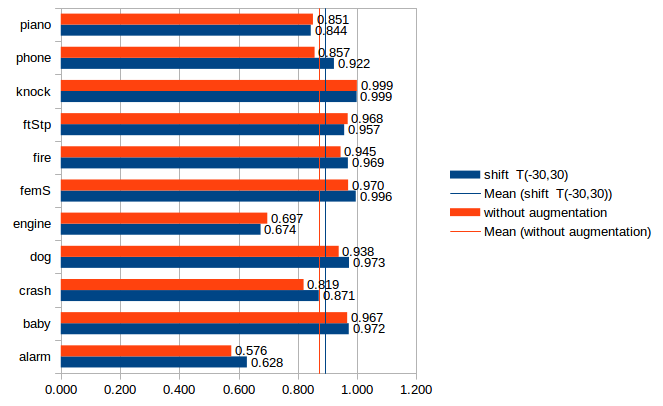
\includegraphics[scale=0.85]{../image/chapter3/bal_acc_T1.png}
\end{figure}

\subsection{Shifting policies}
Besides shifting over time domain, shifting over both frequency domain and time domain is another shifting policy. Shifting over time domain adds the variability of recording delay. Shifting over frequency domain adds the variability of basic frequency of the sound source. These two variability can be both considered as irrelevant.
\begin{figure}[h!]
	\caption{Balanced accuracy of two shifting policies,shift over  T(-30,30),shift over T(-30,30),F(-8,8)}
	\label{fig:balcompare2}
	\centering
	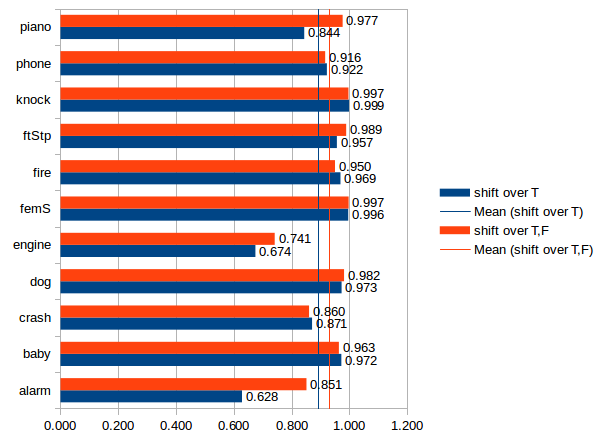
\includegraphics[scale=0.9]{../image/chapter3/bal_acc_TvsF.png}
\end{figure}
The parameter setting for shifting over time domain policy is the same as that described in section \ref{subsec:dataaug}, which is $T(-30,30)$. The parameter setting for shifting over time and frequency domain is $T(-30,30),F(-8,8)$.
 For 6 of the sound types, shifting over time and frequency domain outperforms shifting over time domain. The averaged balanced accuracy over 11 sound types of shifting over time and frequency domain is greater than the other shifting policy. So in the following experiments of shifting parameters, I preferred to adopt the shifting over time and frequency policy.
 
\subsection{Shifting Parameters}
To roughly find a good parameter settings for data augmentation, I carried out three experiments with different parameter settings:
\begin{itemize}
	\item $T(-30,30),F(-8,8)$
	\item $T(-15,15),F(-4,4)$
	\item $T(-40,40),F(-8,8)$
\end{itemize}

 Fig.\ref{fig:balcompare3} shows the balanced accuracy and Fig.\ref{fig:senscompare} shows the sensitivity metric of these three experiments. 
% which means shift steps over time domain in range (-15,15) and shift steps over frequency domain in range (-4,4). 
\begin{figure}[h!]
	\caption{Balanced accuracy of 3 parameter settings}
	\label{fig:balcompare3}
	\centering
	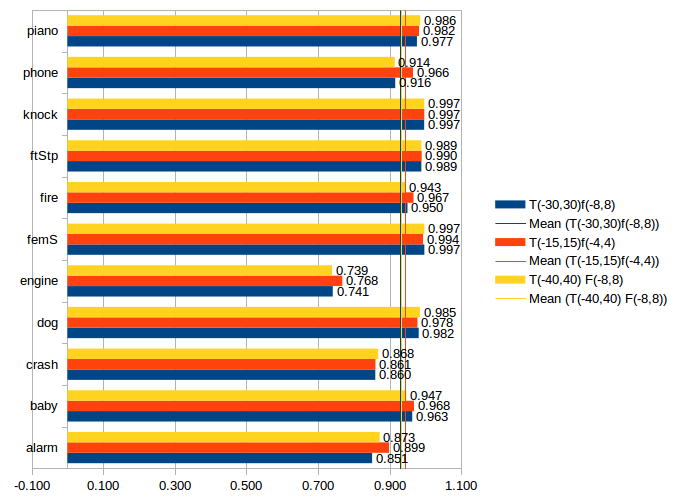
\includegraphics[scale=0.85]{../image/chapter3/bal_params.png}
\end{figure}
\begin{figure}[h!]
	\caption{Sensitivity of 3 parameter settings}
	\label{fig:senscompare}
	\centering
	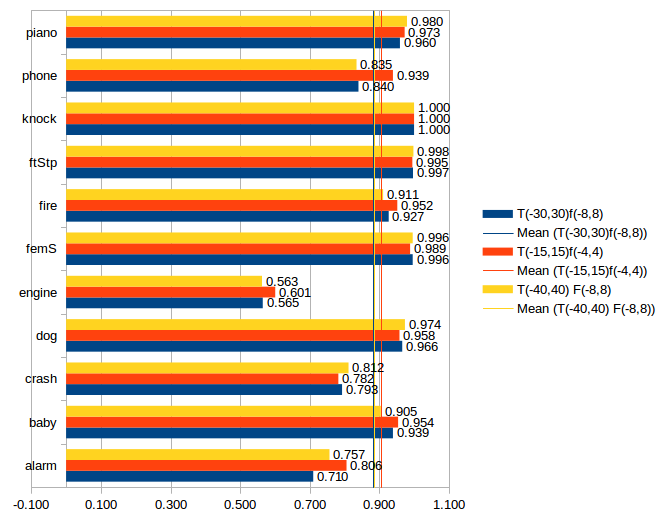
\includegraphics[scale=0.85]{../image/chapter3/sens_params.png}
\end{figure}
From the vertical lines in the diagram, which indicates the mean performance metrics over sound type classes, we can see that the averaged balanced accuracy and the averaged sensitivity of parameter setting $T(-15,15),F(-4,4)$ are the highest among all of these three parameter settings. So currently the  advisable shifting parameters would be $T(-15,15)F(-4,4)$.

\subsection{Summarize and Conclusion}
\label{subsec:sftparams}
The averaged balanced accuracy over 11 sound type classes of the experiments in this chapter are listed in Tab.\ref{tab:balfullresults}. The performance metric values in bold are the best values among these 5 experiments. The best balanced accuracy is acquired in the experiment with data augmentation with parameter setting $T(-15,15)F(-4,4)$.
\begin{table}
\begin{tabular}{|c|c|c|c|}
	\hline		&	\textbf{balanced accuracy}	&	\textbf{sensitivity}	&	\textbf{specificity	}\\
	\hline	\textbf{no data augmentation}	&	0.872	&	0.752	&	\textbf{0.991}	\\
	\hline	\textbf{T(-30,30)}	&	0.891	&	0.799	&	0.984	\\
	\hline	\textbf{T(-30,30),F(-8,8)}	&	0.929	&	0.881	&	0.978	\\
	\hline	\textbf{T(-15,15)F(-4,4)}	&	\textbf{0.943}	&	\textbf{0.905}	&	0.981	\\
	\hline	\textbf{T(-40,40)F(-4,4)}	&	0.931	&	0.885	&	0.977	\\
	\hline 
\end{tabular} 
\label{tab:balfullresults}
\caption{Averaged performance metrics for 5 experiments}
\end{table}
Also if we compare the ROC curves of SigmoidCrossEntropy model from previous chapter and the model with data augmentation constructed in this chapter, we can see that the 'auc'(area under curve) values of SigmoidCrossEntropy model with data augmentation for all of these 11 sound type classes are over $0.95$, while the 'auc' values of SigmoidCrossEntropy model without data augmentation for sound type 'alarm' and 'engine' are below $0.95$.  Thus we can conclude that data augmentation can be adopted as a method to control overfitting problem. The ROC curves are shown in Fig.\ref{fig:rocAug}
\begin{figure}[t!]
	\centering
	\subfigure[SigmoidCrossEntropy model without data augmentation]{
		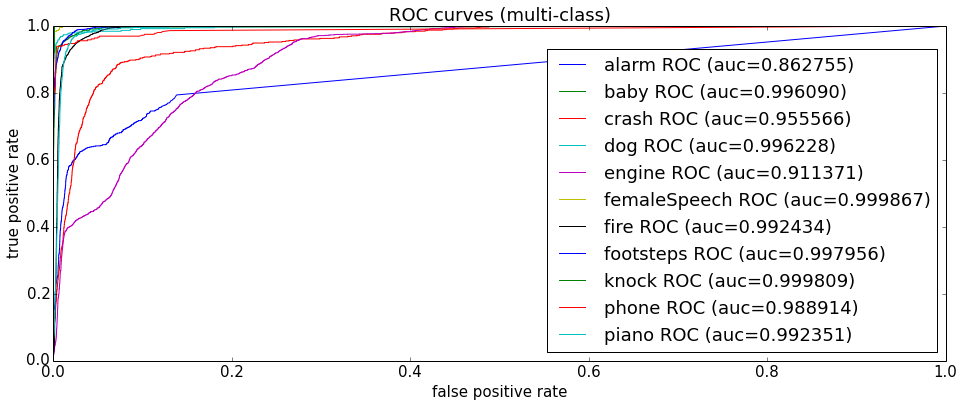
\includegraphics[scale =0.4] {../image/chapter3/rocSCE.png}
		\label{fig:subfig1}
	}
	\subfigure[SigmoidCrossEntropy model with data augmentation $T(-15,15),F(-4,4)$]{
		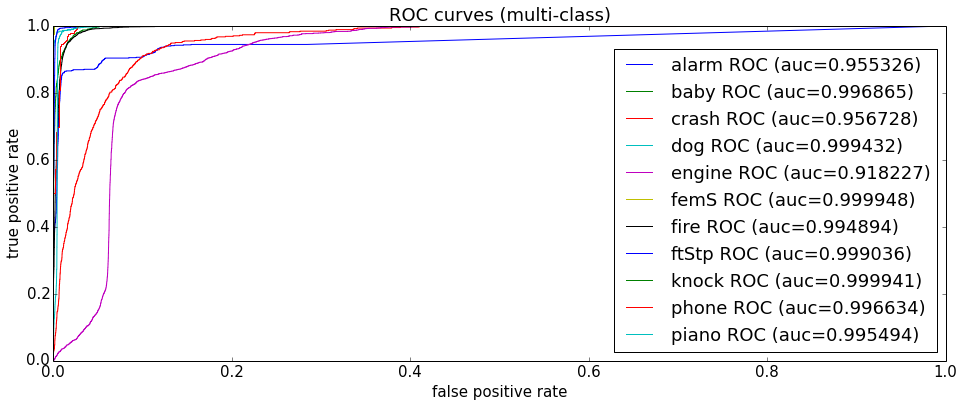
\includegraphics[scale =0.4] {../image/chapter3/rocT15F4.png}
		\label{fig:subfig2}
	}
	\caption{ROC Curves for models with and without Data Augmentation}
	\label{fig:rocAug}
\end{figure}